\documentclass[letterpaper, 12pt]{article}

\usepackage{/Users/zhengz/Desktop/Math/Workspace/Homework1/homework}
\begin{comment}

	
\usepackage{comment} % enables the use of multi-line comments (\ifx \fi) 
\usepackage{lipsum} %This package just generates Lorem Ipsum filler text. 
\usepackage{fullpage} % changes the margin
\usepackage[a4paper, total={7in, 10in}]{geometry}
\usepackage{amsmath}
\usepackage{amssymb,amsthm}  % assumes amsmath package installed
\newtheorem{theorem}{Theorem}
\newtheorem{corollary}{Corollary}
\usepackage{graphicx}
\usepackage{subcaption}
\usepackage{tikz}
\usepackage{capt-of}
\usepackage{multicol}
\usepackage{unicode-math}
\DeclareMathAlphabet\amsmathbb{U}{msb}{m}{n}
\DeclareMathAlphabet\cmmathcal{OMS}{cmsy}{m}{n}
%\setmathfont{Latin Modern Math}
%\setmathfont[range={\mathscr,\mathbfscr}]{XITS Math}
\usepackage{quiver}
\usepackage{setspace}

\usetikzlibrary{arrows}
\usepackage{verbatim}
\usepackage[shortlabels]{enumitem}

\usepackage{float}
\usepackage{tikz-cd}


    
\usepackage{xcolor}
\usepackage{mdframed}
\usepackage[shortlabels]{enumitem}
%\usepackage{indentfirst}
\usepackage{hyperref}
    
\renewcommand{\thesubsection}{\thesection.\alph{subsection}}


\newenvironment{problem}[2][Problem]
    { \begin{mdframed}[backgroundcolor=gray!20] \textbf{#1 #2} \\}
    {  \end{mdframed}}

\newenvironment{background}
{\begin{center}
    \begin{tabular}{|p{\textwidth}|}
    \hline\\
    }
    { 
    \\\\\hline
    \end{tabular} 
    \end{center}}
% Define solution environment
\newenvironment{solution}
    {\textit{Solution:}}
    {}

%Define the claim environment
\newenvironment{claim}[1]{\par\noindent\underline{Claim:}\space#1}{}
\newenvironment{claimproof}[1]{\par\noindent\underline{Proof:}\space#1}{\hfill $\blacksquare$}

%\let\mathbb\oldmathbb

\renewcommand{\qed}{\quad\qedsymbol}
\newcommand{\rank}{\text{rank}\,}
\newcommand{\im}{\text{Im}\,}
\newcommand{\la}{\langle}
\newcommand{\ra}{\rangle}
\renewcommand{\mathbb}{\amsmathbb}
\newcommand{\iif}{\ \ \ \text{if}\ \ \ }
\newcommand{\colim}{\text{colim}}
\newcommand{\otherwise}{\text{otherwise}}
\newcommand{\coker}{\text{coker}\,}
\newcommand{\Aut}{\text{Aut}}
\newcommand{\ti}{\tilde}
\newcommand{\Stab}{\text{Stab}}
	
\end{comment}
%%%%%%%%%%%%%%%%%%%%%%%%%%%%%%%%%%%%%%%%%%%%%%%%%%%%%%%%%%%%%%%%%%%%%%%%%%%%%%%%%%%%%%%%%%%%%%%%%%%%%%%%%%%%%%%%%%%%%%%%%%%%%%%%%%%%%%%%
\begin{document}
%Header-Make sure you update this information!!!!
\noindent
%%%%%%%%%%%%%%%%%%%%%%%%%%%%%%%%%%%%%%%%%%%%%%%%%%%%%%%%%%%%%%%%%%%%%%%%%%%%%%%%%%%%%%%%%%%%%%%%%%%%%%%%%%%%%%%%%%%%%%%%%%%%%%%%%%%%%%%%
\large\textbf{Zhengdong Zhang} \hfill \textbf{Homework 2}   \\
Email: zhengz@uoregon.edu \hfill ID: 952091294 \\
\normalsize Course: MATH 636 - Algebraic Topology III \hfill Term: Spring 2025\\
Instructor: Dr.Daniel Dugger \hfill Due Date: $18^{th}$ April, 2025 \\
\noindent\rule{7in}{2.8pt}
\setstretch{1.1}

%%%%%%%%%%%%%%%%%%%%%%%%%%%%%%%%%%%%%%%%%%%%%%%%%%%%%%%%%%%%%%%%%%%%%%%%%%%%%%%%%%%%%%%%%%%%%%%%%%%%%%%%%%%%%%%%%%%%%%%%%%%%%%%%%%%%%%%%
%Probelm 1 
%%%%%%%%%%%%%%%%%%%%%%%%%%%%%%%%%%%%%%%%%%%%%%%%%%%%%%%%%%%%%%%%%%%%%%%%%%%%%%%%%%%%%%%%%%%%%%%%%%%%%%%%%%%%%%%%%%%%%%%%%%%%%%%%%%%%%%%%
\begin{problem}{1}
Determine all the cohomology groups \(H^*(\mathbb{R}P^4\#\mathbb{C}P^2)\). 
\end{problem}
\begin{solution}
We first use the Mayer-Vietoris sequences in cohomology as follows:
\[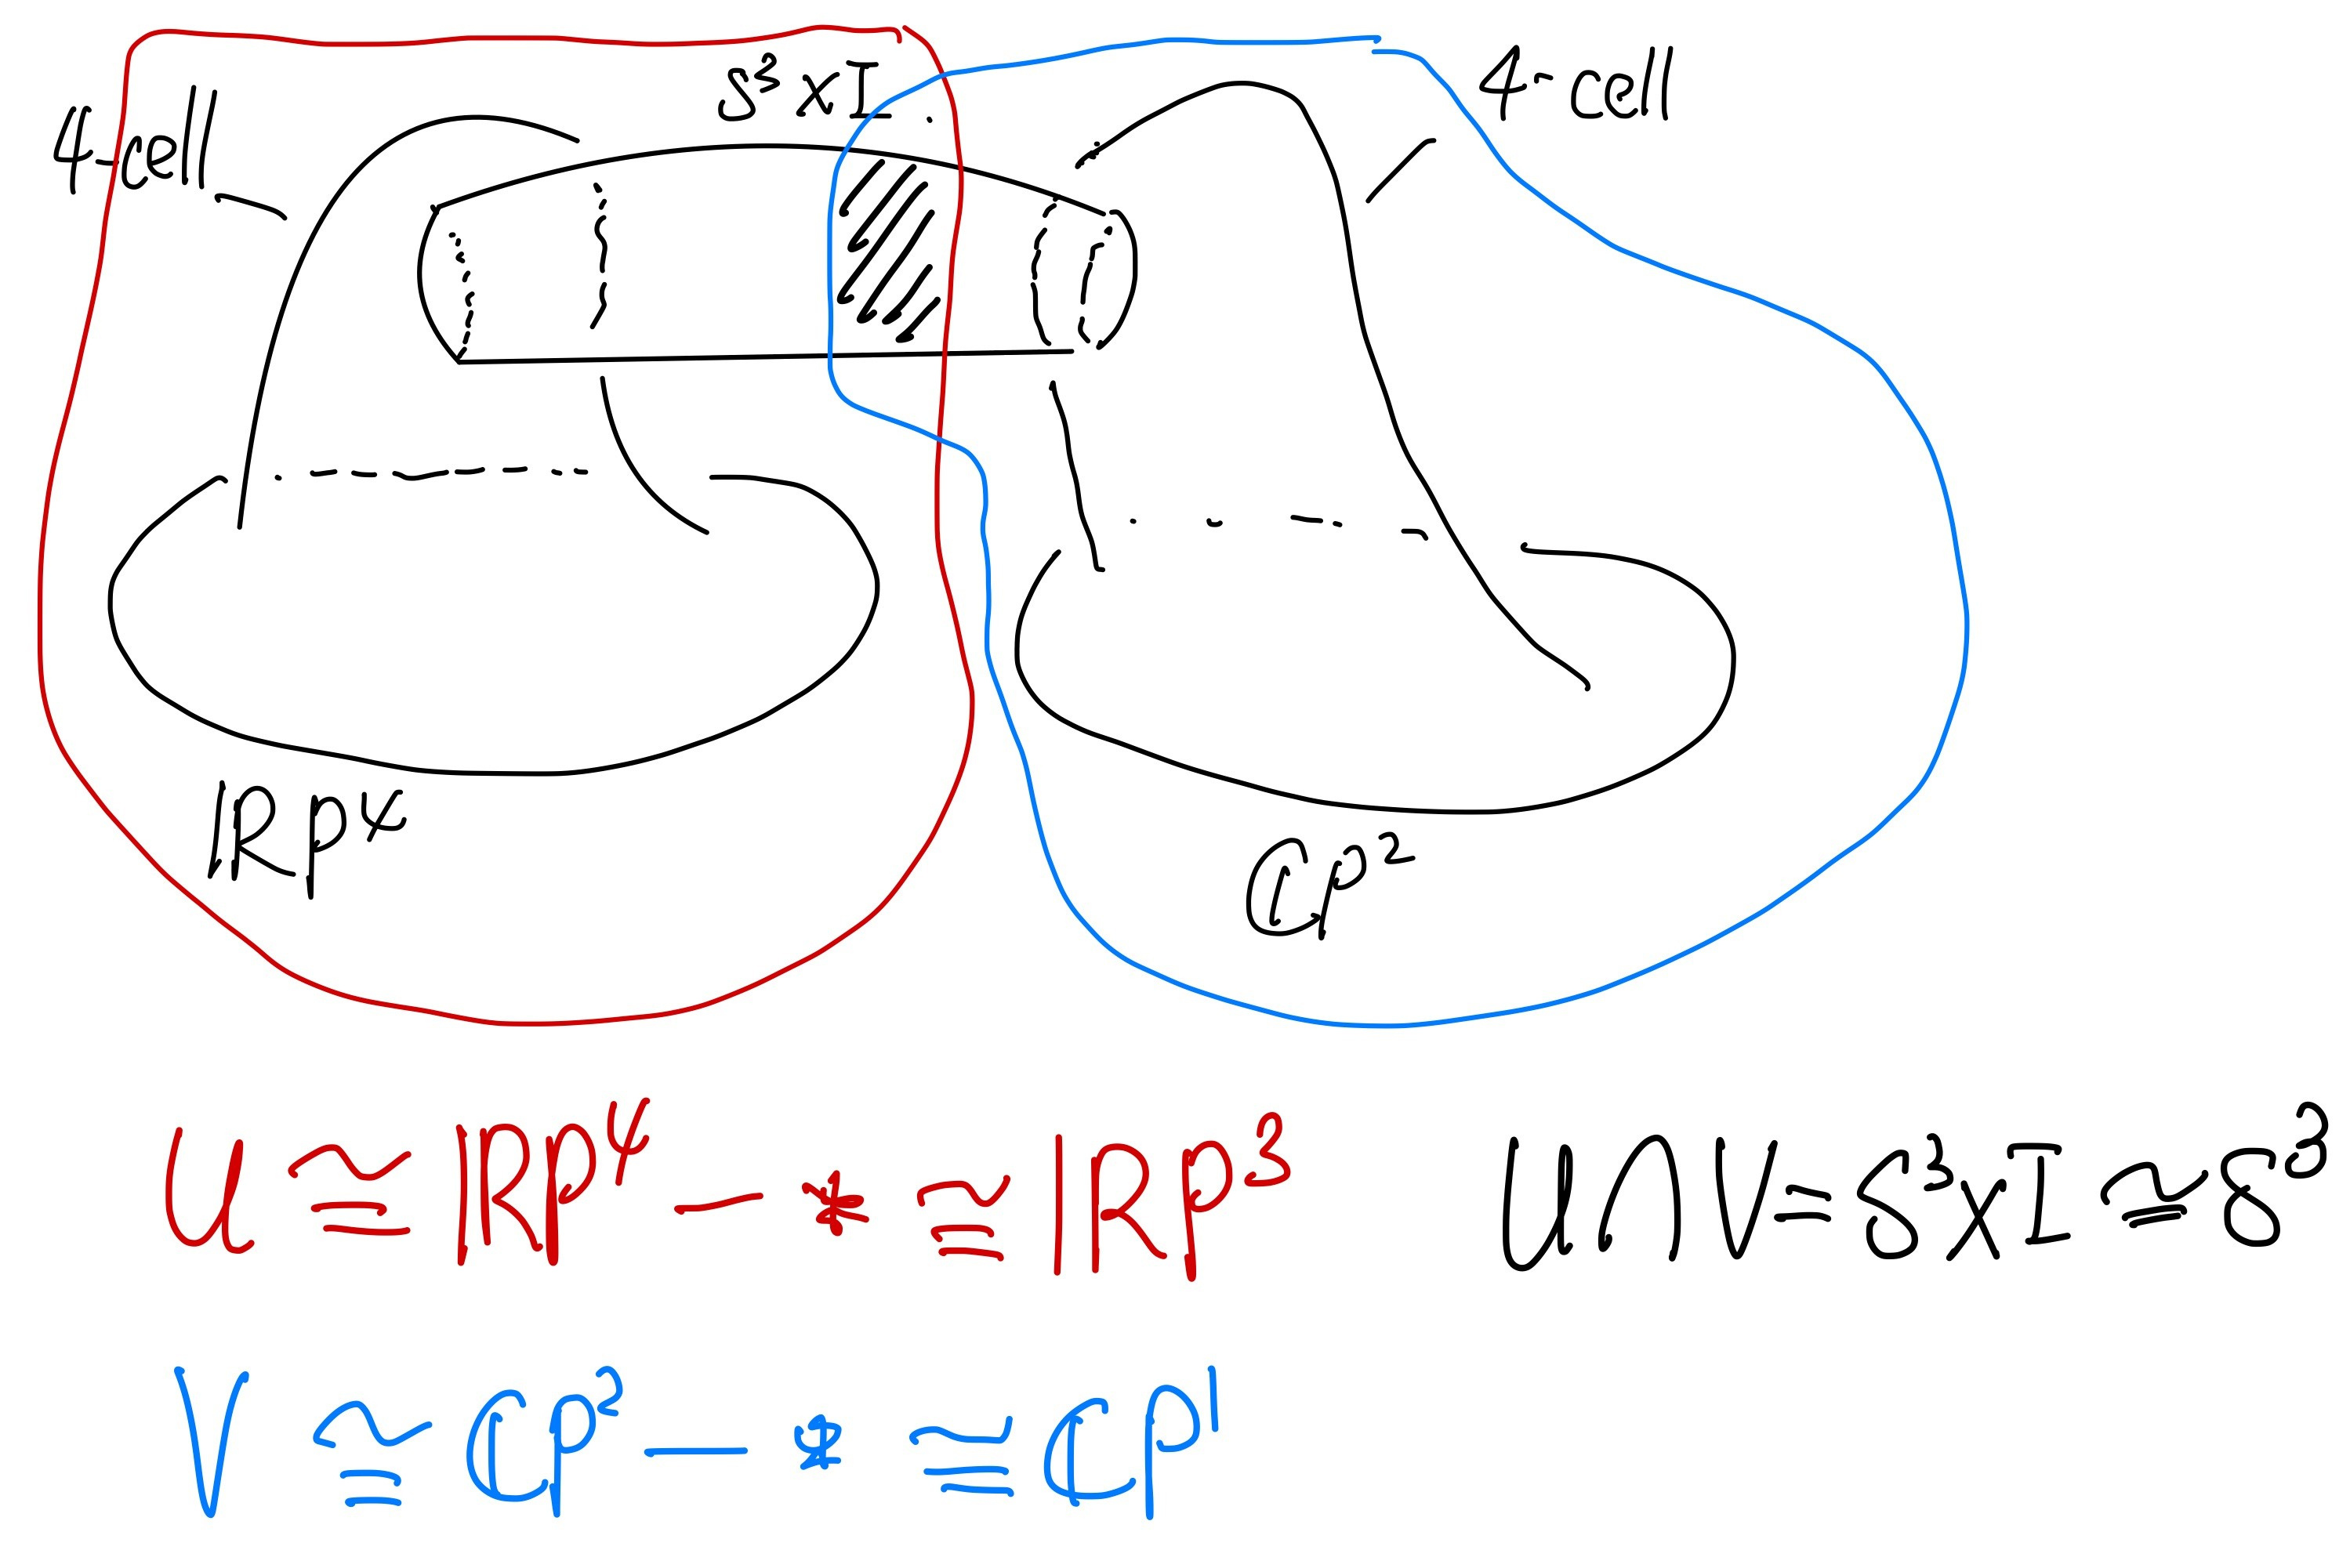
\includegraphics[scale=0.1]{Pictures/HW2-1-1.jpg}\]
Let \(X=\mathbb{R}P^4\#\mathbb{C}P^2\). We have the following long exact sequence in cohomology 
% https://q.uiver.app/#q=WzAsMjMsWzEsMCwiSF4qKFgpIl0sWzIsMCwiSF4qKFxcbWF0aGJie1J9UF4zKVxcb3BsdXMgSF4qKFxcbWF0aGJie0N9UF4xKSJdLFszLDAsIkheKihTXjMpIl0sWzAsMSwiMCJdLFswLDIsIjEiXSxbMCwzLCIyIl0sWzAsNCwiMyJdLFswLDUsIjQiXSxbMSwxLCI/Il0sWzIsMSwiXFxtYXRoYmJ7Wn1cXG9wbHVzIFxcbWF0aGJie1p9Il0sWzMsMSwiXFxtYXRoYmJ7Wn0iXSxbMSwyLCI/Il0sWzEsMywiPyJdLFsxLDQsIj8iXSxbMSw1LCI/Il0sWzIsMiwiMFxcb3BsdXMwIl0sWzMsMiwiMCJdLFszLDQsIlxcbWF0aGJie1p9Il0sWzIsMywiXFxtYXRoYmJ7Wn0vMlxcb3BsdXNcXG1hdGhiYntafSJdLFszLDMsIjAiXSxbMyw1LCIwIl0sWzIsNSwiMCJdLFsyLDQsIlxcbWF0aGJie1p9XFxvcGx1czAiXSxbOCw5XSxbOSwxMF0sWzEwLDExXSxbMTEsMTVdLFsxNSwxNl0sWzE2LDEyXSxbMTIsMThdLFsxOCwxOV0sWzE5LDEzXSxbMTMsMjJdLFsyMiwxN10sWzE3LDE0XSxbMTQsMjFdLFsyMSwyMF1d
\[\begin{tikzcd}
	& {H^*(X)} & {H^*(\mathbb{R}P^3)\oplus H^*(\mathbb{C}P^1)} & {H^*(S^3)} \\
	0 & {?} & {\mathbb{Z}\oplus \mathbb{Z}} & {\mathbb{Z}} \\
	1 & {?} & {0\oplus0} & 0 \\
	2 & {?} & {\mathbb{Z}/2\oplus\mathbb{Z}} & 0 \\
	3 & {?} & {\mathbb{Z}\oplus0} & {\mathbb{Z}} \\
	4 & {?} & 0 & 0
	\arrow[from=2-2, to=2-3]
	\arrow[from=2-3, to=2-4]
	\arrow[from=2-4, to=3-2]
	\arrow[from=3-2, to=3-3]
	\arrow[from=3-3, to=3-4]
	\arrow[from=3-4, to=4-2]
	\arrow[from=4-2, to=4-3]
	\arrow[from=4-3, to=4-4]
	\arrow[from=4-4, to=5-2]
	\arrow[from=5-2, to=5-3]
	\arrow[from=5-3, to=5-4]
	\arrow[from=5-4, to=6-2]
	\arrow[from=6-2, to=6-3]
	\arrow[from=6-3, to=6-4]
\end{tikzcd}\]
Note that \(X\) is connected, so \(H^0(X)=\mathbb{Z}\). By exactness of the above sequence, we have 
\[H^2(X)\cong \mathbb{Z}\oplus \mathbb{Z}/2.\]
Now consider collapsing the \(\mathbb{C}P^1\subseteq \mathbb{C}P^2\) in \(X\) as shown 
\[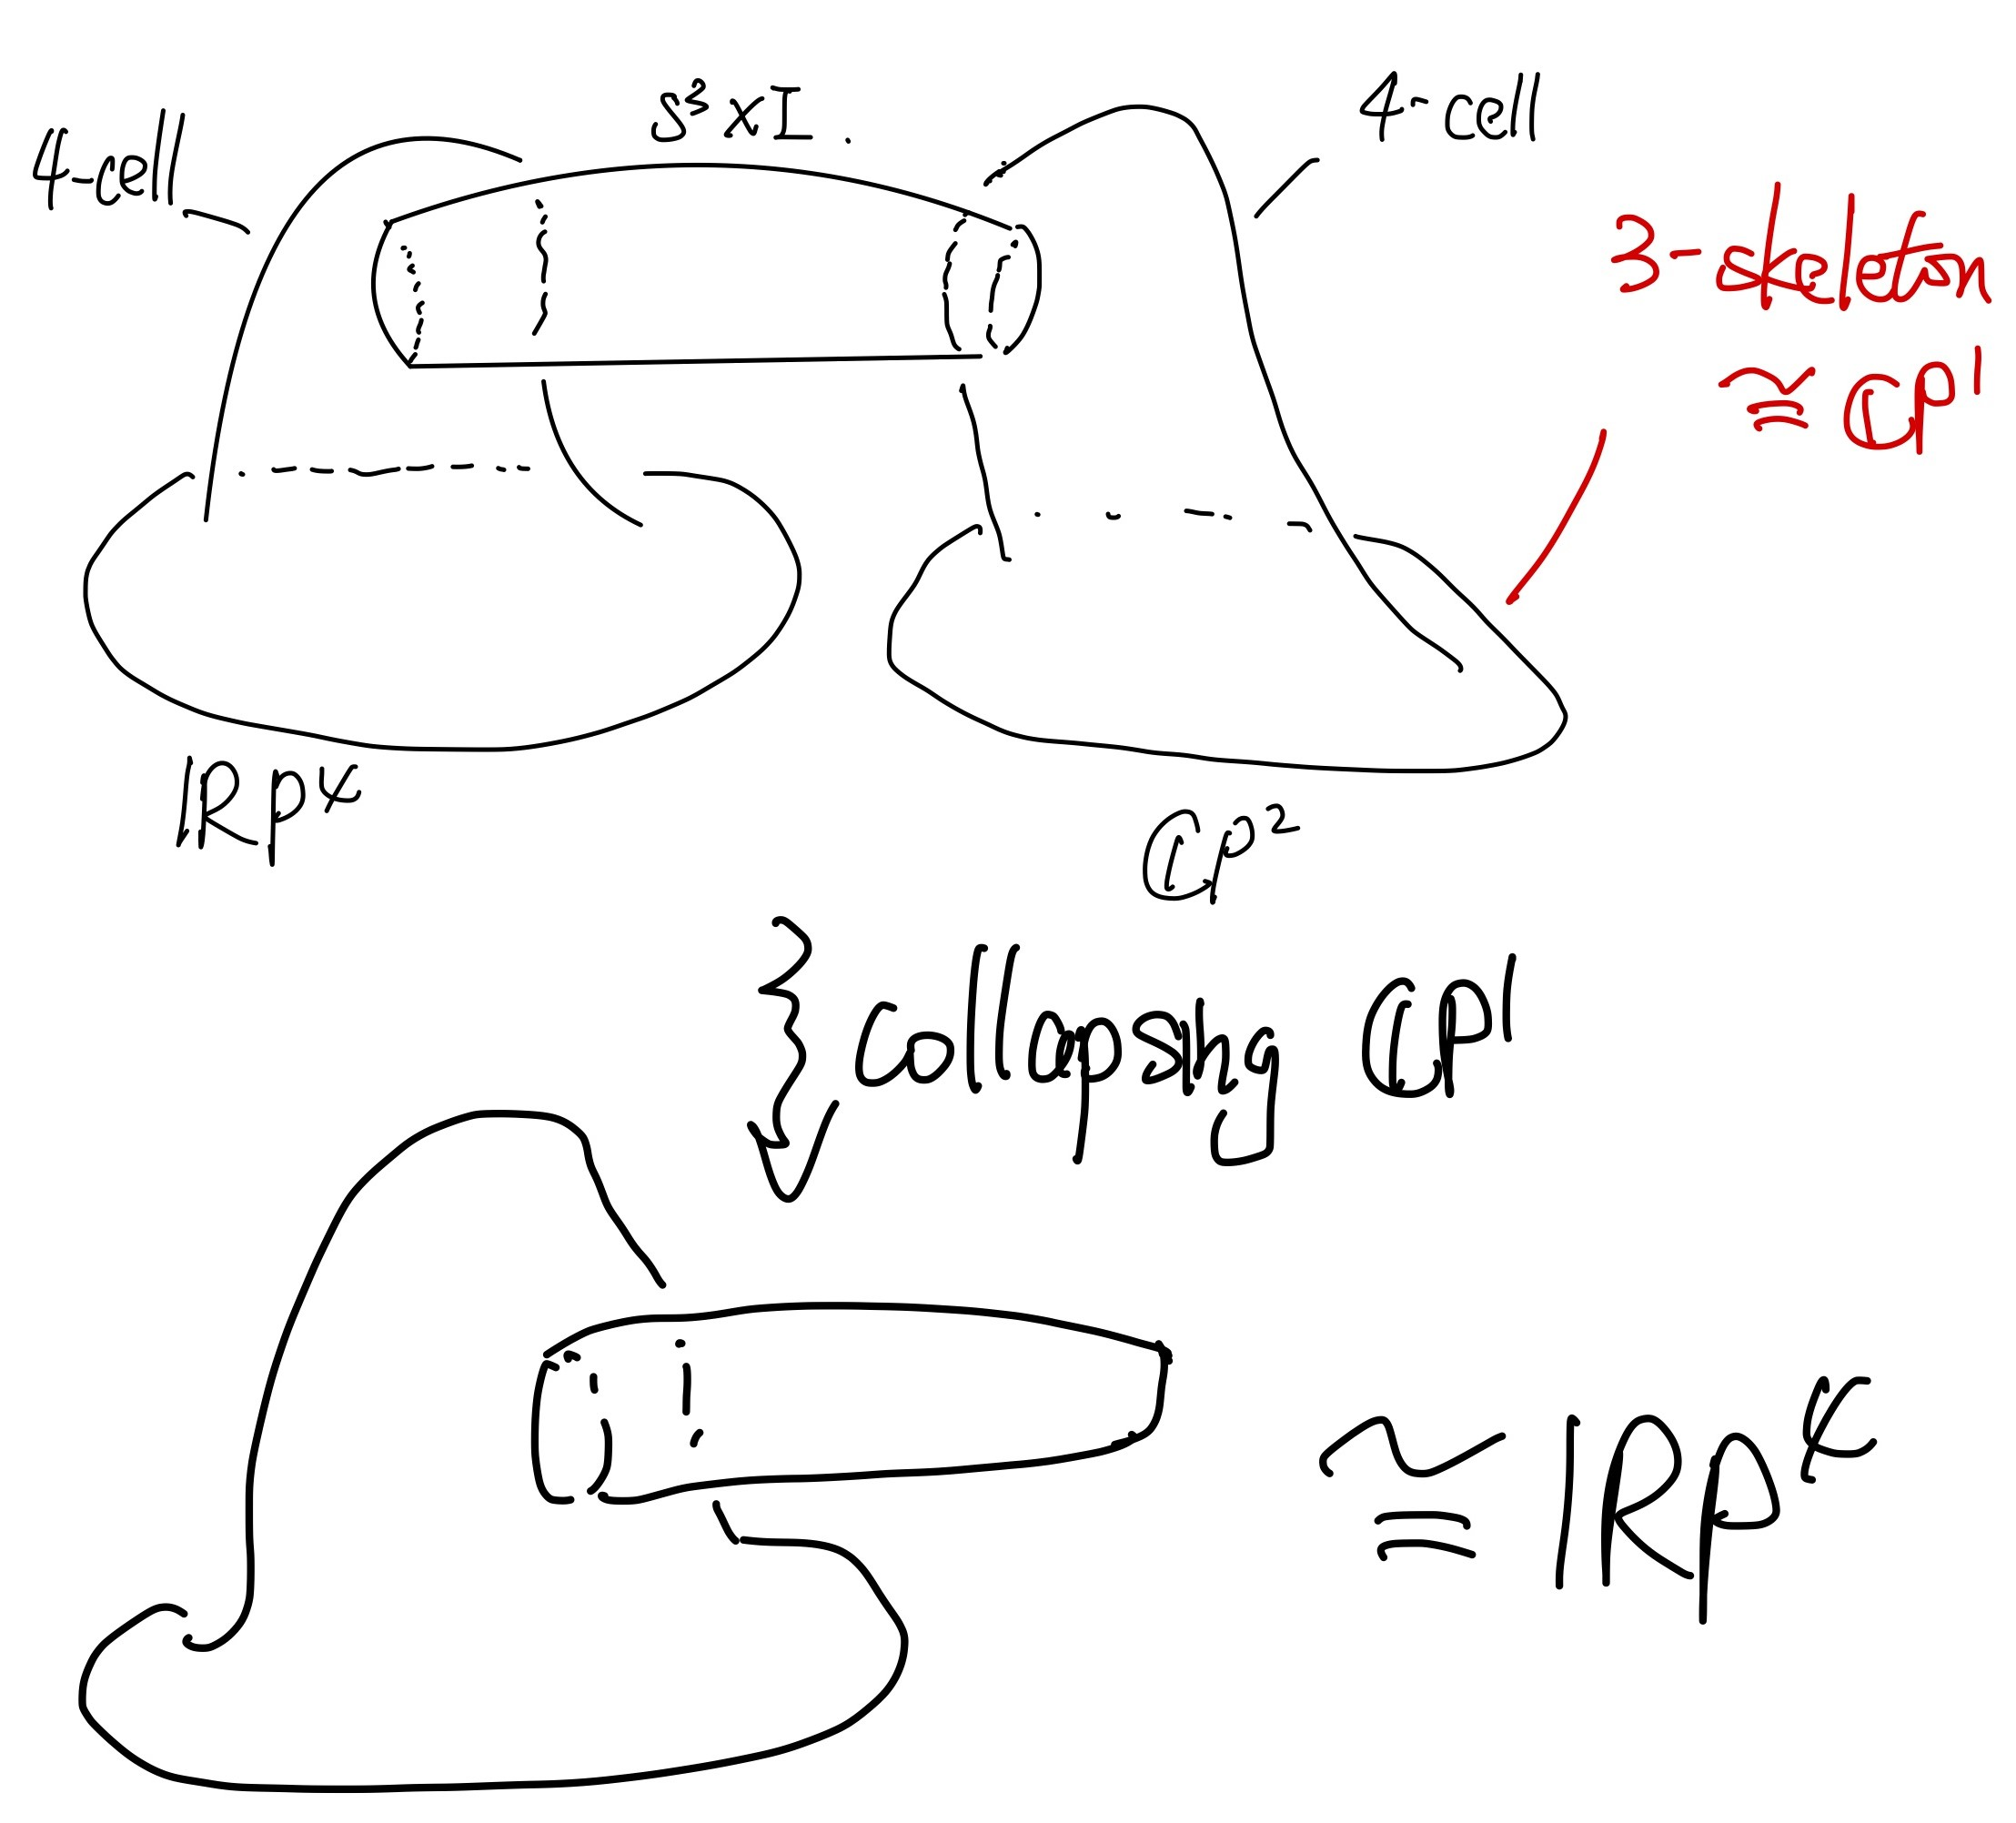
\includegraphics[scale=0.1]{Pictures/HW2-1-2.jpg}\]
we have a cofiber sequence 
\[\mathbb{C}P^1\rightarrow X\rightarrow \mathbb{R}P^4\]
This gives us a long exactness sequence in reduced cohomology
% https://q.uiver.app/#q=WzAsMjMsWzEsMCwiXFx0aWxkZXtIfV4qKFxcbWF0aGJie1J9UF40KSJdLFsyLDAsIlxcdGlsZGV7SH1eKihYKSJdLFszLDAsIlxcdGlsZGV7SH1eKihcXG1hdGhiYntDfVBeMSkiXSxbMCwxLCIwIl0sWzAsMiwiMSJdLFswLDMsIjIiXSxbMCw0LCIzIl0sWzAsNSwiNCJdLFsyLDEsIjAiXSxbMSwxLCIwIl0sWzMsMSwiMCJdLFsxLDIsIjAiXSxbMSwzLCJcXG1hdGhiYntafS8yIl0sWzEsNCwiMCJdLFsxLDUsIlxcbWF0aGJie1p9LzIiXSxbMywzLCJcXG1hdGhiYntafSJdLFszLDIsIjAiXSxbMyw0LCIwIl0sWzMsNSwiMCJdLFsyLDIsIj8iXSxbMiwzLCJcXG1hdGhiYntafVxcb3BsdXNcXG1hdGhiYntafS8yIl0sWzIsNCwiPyJdLFsyLDUsIj8iXSxbOSw4XSxbOCwxMF0sWzEwLDExXSxbMTEsMTldLFsxOSwxNl0sWzE2LDEyXSxbMTIsMjBdLFsyMCwxNV0sWzE1LDEzXSxbMTMsMjFdLFsyMSwxN10sWzE3LDE0XSxbMTQsMjJdLFsyMiwxOF1d
\[\begin{tikzcd}
	& {\tilde{H}^*(\mathbb{R}P^4)} & {\tilde{H}^*(X)} & {\tilde{H}^*(\mathbb{C}P^1)} \\
	0 & 0 & 0 & 0 \\
	1 & 0 & {?} & 0 \\
	2 & {\mathbb{Z}/2} & {\mathbb{Z}\oplus\mathbb{Z}/2} & {\mathbb{Z}} \\
	3 & 0 & {?} & 0 \\
	4 & {\mathbb{Z}/2} & {?} & 0
	\arrow[from=2-2, to=2-3]
	\arrow[from=2-3, to=2-4]
	\arrow[from=2-4, to=3-2]
	\arrow[from=3-2, to=3-3]
	\arrow[from=3-3, to=3-4]
	\arrow[from=3-4, to=4-2]
	\arrow[from=4-2, to=4-3]
	\arrow[from=4-3, to=4-4]
	\arrow[from=4-4, to=5-2]
	\arrow[from=5-2, to=5-3]
	\arrow[from=5-3, to=5-4]
	\arrow[from=5-4, to=6-2]
	\arrow[from=6-2, to=6-3]
	\arrow[from=6-3, to=6-4]
\end{tikzcd}\]
By exactness, we know \(H^1(X)=H^3(X)=0\) and \(H^4(X)=\mathbb{Z}/2\). We can summarize the cohomology groups as follows.
\[H^i(\mathbb{R}P^4\#\mathbb{C}P^2)=\begin{cases}
    \mathbb{Z},&\iif i=0;\\ 
    \mathbb{Z}/2,&\iif i=4;\\ 
    \mathbb{Z}\oplus \mathbb{Z}/2,&\iif i=2;\\
    0,&\otherwise.
\end{cases}\]
\end{solution}

\noindent\rule{7in}{2.8pt}
%%%%%%%%%%%%%%%%%%%%%%%%%%%%%%%%%%%%%%%%%%%%%%%%%%%%%%%%%%%%%%%%%%%%%%%%%%%%%%%%%%%%%%%%%%%%%%%%%%%%%%%%%%%%%%%%%%%%%%%%%%%%%%%%%%%%%%%%
%Probelm 2
%%%%%%%%%%%%%%%%%%%%%%%%%%%%%%%%%%%%%%%%%%%%%%%%%%%%%%%%%%%%%%%%%%%%%%%%%%%%%%%%%%%%%%%%%%%%%%%%%%%%%%%%%%%%%%%%%%%%%%%%%%%%%%%%%%%%%%%%
\begin{problem}{2}
Let \(f:X\rightarrow Y\) be a map, and consider the diagram 
% https://q.uiver.app/#q=WzAsNCxbMCwwLCJIXmsoWTtSKSJdLFsyLDAsIkheayhYO1IpIl0sWzAsMSwiXFxob20oSF9rKFkpLFIpIl0sWzIsMSwiXFxob20oSF9rKFgpLFIpIl0sWzIsMywiXFxob20oZl8qLFIpIl0sWzAsMiwiXFxwaGkiXSxbMSwzLCJcXHBoaSIsMl0sWzAsMSwiZl4qIl1d
\[\begin{tikzcd}
	{H^k(Y;R)} && {H^k(X;R)} \\
	{\hom(H_k(Y),R)} && {\hom(H_k(X),R)}
	\arrow["{f^*}", from=1-1, to=1-3]
	\arrow["\phi", from=1-1, to=2-1]
	\arrow["\phi"', from=1-3, to=2-3]
	\arrow["{\hom(f_*,R)}", from=2-1, to=2-3]
\end{tikzcd}\]
where the bottom horizontal map is the one obtained by applying the functor \(\hom(-,R)\) to \(f_*:H_k(X)\rightarrow H_k(Y)\). Here the vertical maps \(\phi\) are the adjoints to the Kronecker pairings, namely 
the maps that send a cohomology class \([\alpha]\) to the homomorphism \([v]\mapsto \alpha(v)\). Verify that the above diagram commutes. 
\end{problem}
\begin{solution}
Let \(\alpha:C_k(Y)\rightarrow R\) be a cocycle in \(Y\) and \([\alpha]\) be the cohomology class represented by \(\alpha\) in \(H^k(Y;R)\). By definition, we know that \(f^*([\alpha])=[\alpha\circ f_\#]\), where 
\(f_\#:C_k(X)\rightarrow C_k(Y)\) is the map on the chain complex induced by \(f\). By definition, \(\phi\) sends \([\alpha\circ f_\#]\) to the homomorphism \([v]\mapsto (\alpha\circ f_\#)(v)\) for any \(k\)-cycle \(v\in C_k(X)\). On the other hand, 
\(\phi\) sends \([\alpha]\) to the homomorphism \([w]\mapsto \alpha(w)\) for any \(k\)-cycle \(w\in C_k(Y)\). Applying \(\hom(f_*,R)\) to this homomorphism, we obtain a homomorphism sending any \([v]\in H_k(X)\) to 
\(\alpha(f_*([v]))\). Note that by definition, for any \(k\)-cycle \(v\in C_k(X)\), we have 
\[\alpha(f_*([v]))=\alpha([f_\#(v)])=\alpha(f_\#(v))=(\alpha\circ f_\#)(v).\]
This proves the commutativity of this diagram. 
\end{solution}

\noindent\rule{7in}{2.8pt}
%%%%%%%%%%%%%%%%%%%%%%%%%%%%%%%%%%%%%%%%%%%%%%%%%%%%%%%%%%%%%%%%%%%%%%%%%%%%%%%%%%%%%%%%%%%%%%%%%%%%%%%%%%%%%%%%%%%%%%%%%%%%%%%%%%%%%%%%
%Probelm 3
%%%%%%%%%%%%%%%%%%%%%%%%%%%%%%%%%%%%%%%%%%%%%%%%%%%%%%%%%%%%%%%%%%%%%%%%%%%%%%%%%%%%%%%%%%%%%%%%%%%%%%%%%%%%%%%%%%%%%%%%%%%%%%%%%%%%%%%%
\begin{problem}{3}
\begin{enumerate}[(a)]
\item Give a \(\Delta\)-complex structure on \(\mathbb{R}P^2\) and use this to write down explicit cocycles \(\alpha\in Z^1(\mathbb{R}P^2;\mathbb{Z}/2)\) and 
\(\beta\in Z^2(\mathbb{R}P^2;\mathbb{Z}/2)\) that generates the cohomology groups. Compute \(\alpha\cup \alpha\) and decide if it equals \(\beta\) or not in \(H^*(\mathbb{R}P^2;\mathbb{Z}/2)\). 
\item Let \(K\) be the Klein bottle. Write down explicit cocycles whcih represent generators for \(H^*(K;\mathbb{Z}/2)\) and use these to compute all the cup products of these generators. 
\item If \(R\) is a ring then we can extend the Kronecker pairing to be maps 
\[H^k(X;R)\otimes H_k(X;R)\rightarrow R.\]
The adjoint is then a map 
\[\phi_R:H^k(X;R)\rightarrow \hom(H_k(X),R).\]
When \(X\) is the Klein bottle and \(\mathbb{R}=\mathbb{Z}/2\) determine bases for each \(H^k(X;R)\) and verify by hand that the maps \(\phi\) are isomorphisms for all \(k\). 
\end{enumerate}
\end{problem}
\begin{solution}
\begin{enumerate}[(a)]
\item Consider the following \(\Delta\)-complex structure for \(\mathbb{R}P^2\):
\[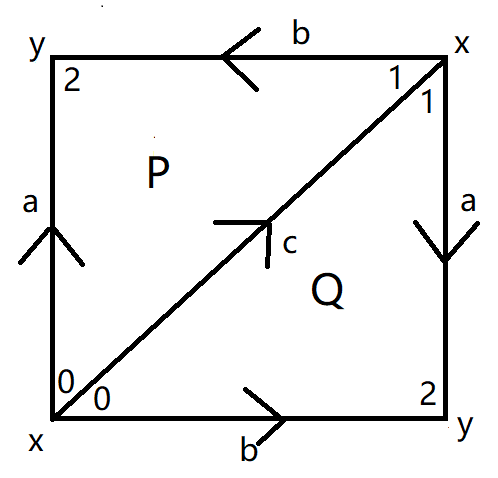
\includegraphics[scale=0.4]{Pictures/HW2-3-1.png}\]
We know from last homework that \(H^1(\mathbb{R}P^2;\mathbb{Z}/2)=H^2(\mathbb{R}P^2;\mathbb{Z}/2)=\mathbb{Z}/2\). So as long as the cocycle \(\alpha,\beta\in Z^*(\mathbb{R}P^2;\mathbb{Z}/2)\) are not zero, they are the generator of the cohomology groups. 
Consider \(\hat{a}+\hat{c}\in C^1(\mathbb{R}P^2;\mathbb{Z}/2)\), we check that this is a cocycle.
\begin{align*}
    (\delta(\hat{a}+\hat{c}))(P)&=(\hat{a}+\hat{c})(\partial P)=(\hat{a}+\hat{c})(-a+b+c)=1+1=0;\\ 
    (\delta(\hat{a}+\hat{c}))(Q)&=(\hat{a}+\hat{c})(\partial Q)=(\hat{a}+\hat{c})(a-b+c)=1+1=0.
\end{align*}
This proves \(\hat{a}+\hat{c}\in Z^1(\mathbb{R}P^2;\mathbb{Z}/2)\) and we need to show that \(\hat{a}+\hat{c}\) is not a coboundary, this is true because
\begin{align*}
    \delta(\hat{x})(a)&=\delta(\hat{y})(a)=1,\\ 
    \delta(\hat{x})(b)&=\delta(\hat{y})(b)=1,\\ 
    \delta(\hat{x})(c)&=\delta(\hat{y})(c)=0.
\end{align*}
So \(\hat{a}+\hat{c}\) cannot be realized as the image of \(C^0(\mathbb{R}P^2;\mathbb{Z}/2)\). This implies that 
\(\alpha=[\hat{a}+\hat{c}]\) generates the cohomology group \(H^1(\mathbb{R}P^2;\mathbb{Z}/2)=\mathbb{Z}/2\). Note that \(\mathbb{R}P^2\) does not have 
\(3\)-simplices, and we know \(H^2(\mathbb{R}P^2;\mathbb{Z}/2)=\mathbb{Z}/2\), so \(\hat{Q}\in Z^2(\mathbb{R}P^2;\mathbb{Z}/2)\) and note that 
\[\partial P=\partial Q=a+b+c.\]
So \(\hat{Q}\) is not a coboundary because \(\hat{Q}(P)=0\) and \(\hat{Q}(Q)=1\). This implies that 
\(\beta=[\hat{Q}]\) generates \(H^2(\mathbb{R}P^2;\mathbb{Z}/2)\). Next, we calculate the cup product. 
\begin{align*}
    (\alpha\cup \alpha)(P)&=\alpha(c)\cdot \alpha(b)=0;\\ 
    (\alpha\cup \alpha)(Q)&=\alpha(c)\cdot \alpha(a)=1.
\end{align*}
This proves that \((\hat{a}+\hat{c})\cup(\hat{a}+\hat{c})=\hat{Q}\) on the chain level and in the cohomology ring \(H^*(\mathbb{R}P^2;\mathbb{Z}/2)\), we have \(\alpha\cup\alpha=\beta\).
\item Consider the cellular chain complex of the Klein bottle \(K\)
\[0\rightarrow \mathbb{Z}\xrightarrow{\begin{pmatrix}
2\\ 
0
\end{pmatrix}}\mathbb{Z}^2\xrightarrow{0}\mathbb{Z}\rightarrow 0\]
Apply \(\hom(-,\mathbb{Z}/2)\), we obtain the cellular cochain complex 
\[0\leftarrow\mathbb{Z}/2\xleftarrow{0} (\mathbb{Z}/2)^2\xleftarrow{0}\mathbb{Z}/2\leftarrow 0.\]
So we know \(H^0(K;\mathbb{Z}/2)=H^2(K;\mathbb{Z}/2)=\mathbb{Z}/2\), each has one generator and \(H^1(K;\mathbb{Z}/2)=(\mathbb{Z}/2)^2\) having two generators. Consider the following \(\Delta\)-complex structure of \(K\)
\[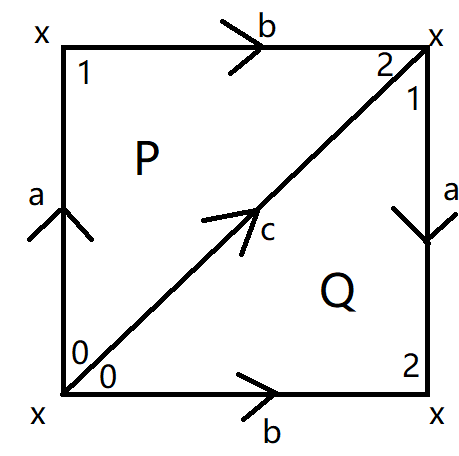
\includegraphics[scale=0.4]{Pictures/HW2-3-2.png}\]
\(K\) only has one \(0\)-simplex \(x\), so the cocycle \(\hat{x}\) generates \(H^0(K;\mathbb{Z}/2)\). \(K\) has no \(3\)-simplices, so \(\hat{P}\) is a cocycle and we need to show that 
\(\hat{P}\) is not a coboundary. Suppose \(\delta(m\hat{a}+n\hat{b}+k\hat{c})=\hat{P}\). Then 
\begin{align*}
    1&=(m\hat{a}+n\hat{b}+k\hat{c})(P)=(m\hat{a}+n\hat{b}+k\hat{c})(a+b-c)=m+n+k,\\ 
    0&=(m\hat{a}+n\hat{b}+k\hat{c})(Q)=(m\hat{a}+n\hat{b}+k\hat{c})(a-b+c)=m+n+k.
\end{align*}
This leads to a contradiction and thus \(\hat{P}\) is not a coboundary and generates \(H^2(K;\mathbb{Z}/2)\). Note that 
\begin{align*}
    \partial P&=a+b-c,\\ 
    \partial Q&=a-b+c.
\end{align*}
Consider two cochains \(\alpha=\hat{a}+\hat{b}\) and \(\beta=\hat{a}+\hat{c}\), they are cocycles because 
\begin{align*}
    0=&(\delta\alpha)(P)=(\delta\alpha)(Q),\\
    0=&(\delta\beta)(P)=(\delta\beta)(Q).
\end{align*}
We need to show that \([\alpha]\neq [\beta]\) in \(H^1(K;\mathbb{Z}/2)\). Assume the opposite. This means \(\alpha-\beta\) is a coboundary. We only have one \(0\)-simplex, so 
\(\alpha-\beta=\hat{b}+\hat{c}=\delta\hat{x}\). But 
\[1=(\hat{b}+\hat{c})(b)=(\delta\hat{x})(b)=\hat{x}(x-x)=0\]
A contradiction. This tells us \(\alpha,\beta\) generates \(H^1(K;\mathbb{Z}/2)\). 

Next, we calculate the cup product. For dimension reasons, we have \([\hat{P}]\cup[\hat{P}]=0\), and \([\hat{x}]\) is the unity in the cohomology ring. In degree 1, 
\begin{align*}
    (\alpha\cup\alpha)(P)&=\alpha(a)\cdot \alpha(b)=1\cdot 1=1;\\ 
    (\alpha\cup \alpha)(Q)&=\alpha(c)\cdot \alpha(a)=0\cdot 1=0.
\end{align*}
This tells us \(\alpha\cup\alpha=\hat{P}\) on the cochain level. So 
\[[\alpha]\cup [\alpha]=[\hat{P}].\]
\begin{align*}
    (\beta\cup \beta)(P)&=\beta(a)\cdot \beta(b)=1\cdot 0=0;\\ 
    (\beta\cup \beta)(Q)&=\beta(c)\cdot \beta(a)=1\cdot 1=1.
\end{align*} 
This tells us \(\beta\cup\beta=\hat{Q}\) on the cochain level, and we know that 
\begin{align*}
    \delta(\hat{a}+\hat{b}+\hat{c})(P)&=(\hat{a}+\hat{b}+\hat{c})(a+b-c)=1+1+1=1,\\ 
    \delta(\hat{a}+\hat{b}+\hat{c})(Q)&=(\hat{a}+\hat{b}+\hat{c})(a-b+c)=1+1+1=1.
\end{align*}
This implies \(\hat{P}+\hat{Q}\) is a coboundary and \([\hat{P}]=[\hat{Q}]\) in \(H^2(K;\mathbb{Z}/2)\). So 
\[[\beta]\cup[\beta]=[\hat{P}].\]
\begin{align*}
    (\alpha\cup\beta)(P)&=\alpha(a)\cdot \beta(b)=1\cdot 0=0;\\ 
    (\alpha\cup \beta)(Q)&=\alpha(c)\cdot \beta(a)=0\cdot 1=0.
\end{align*}
This tells us \(\alpha\cup \beta=0\) on the cochain level, so 
\[[\alpha]\cup[\beta]=-([\beta]\cup [\alpha])=0.\]
\item Let \(K\) be the Klein bottle. Consider the \(\Delta\)-complex structure we used in (b)
\[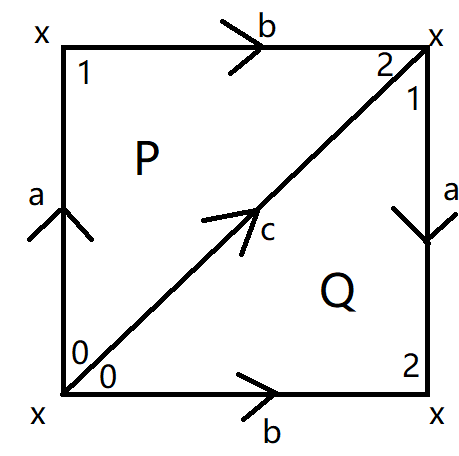
\includegraphics[scale=0.4]{Pictures/HW2-3-2.png}\]
We have a chain complex with \(\mathbb{Z}/2\)-coefficients 
\[0\rightarrow (\mathbb{Z}/2)^2\xrightarrow{d}(\mathbb{Z}/2)^3\xrightarrow{0}\mathbb{Z}/2\rightarrow 0\]
where the boundary map \(d\) is given by the matrix \(\begin{pmatrix}
    1&1\\ 
    1&1\\ 
    1&1
\end{pmatrix}\). So \(H_2(K;\mathbb{Z}/2)=\ker d\) is generated by the 2-cycle \(P+Q\) and \(H_1(K;\mathbb{Z}/2)\) is generated by \(a,b\) where \(c=a+b\). \(H_0(K;\mathbb{Z}/2)\) is generated by \(x\). Note that to check 
\(\phi\) is an isomorphism, it is the same as checking the Kronecker pairing is a perfect pairing. For \(k=0\) and \(k=2\), it is easy to see because on the only generator, we have 
\begin{align*}
    ([\hat{x}],[x])&=\hat{x}(x)=1,\\ 
    ([\hat{P}],P+Q)&=\hat{P}(P+Q)=1.
\end{align*}
For \(k=1\), use \(\alpha=\hat{a}+\hat{b}\) and \(\beta=\hat{a}+\hat{c}\) as generators of \(H^1(K;\mathbb{Z}/2)\) as before, we have 
\begin{align*}
    ([\alpha],[a])&=(\hat{a}+\hat{b})(a)=1,\\ 
    ([\alpha],[b])&=(\hat{a}+\hat{b})(b)=1,\\ 
    ([\beta],[a])&=(\hat{a}+\hat{c})(a)=1,\\ 
    ([\beta],[b])&=(\hat{a}+\hat{c})(b)=0.
\end{align*}
This can be written as a matrix 
\[\begin{pmatrix}
    1&1\\ 
    1&0
\end{pmatrix}\]
which is invertible in \(M_2(\mathbb{Z}/2)\), so this is also a perfect pairing. Thus, we have proved that \(H^k(K;\mathbb{Z}/2)\rightarrow \hom(H_k(K;\mathbb{Z}/2),\mathbb{Z}/2)\) is an isomorphism for \(k=0,1,2\).
\end{enumerate}
\end{solution}

\noindent\rule{7in}{2.8pt}
%%%%%%%%%%%%%%%%%%%%%%%%%%%%%%%%%%%%%%%%%%%%%%%%%%%%%%%%%%%%%%%%%%%%%%%%%%%%%%%%%%%%%%%%%%%%%%%%%%%%%%%%%%%%%%%%%%%%%%%%%%%%%%%%%%%%%%%%
%Probelm 4
%%%%%%%%%%%%%%%%%%%%%%%%%%%%%%%%%%%%%%%%%%%%%%%%%%%%%%%%%%%%%%%%%%%%%%%%%%%%%%%%%%%%%%%%%%%%%%%%%%%%%%%%%%%%%%%%%%%%%%%%%%%%%%%%%%%%%%%%
\begin{problem}{4}
Prove that there does not exist a map \(S^2\rightarrow T\) that induces an isomorphism on \(H_2\). In fact, prove this in two different ways: 
give a proof that uses homotopy groups and give a proof that uses cohomology and the cup product. 
\end{problem}
\begin{solution}
In (1) we prove this using homotopy groups and in (2), we prove this using cohomology rings. 
\begin{enumerate}[(1)]
\item We check that the Hurewicz homomorphism is natural.
\begin{claim}
\(f:X\rightarrow Y\) is a map of connected, pointed spaces. For \(n\geq 1\), we have a commutative diagram 
% https://q.uiver.app/#q=WzAsNCxbMCwwLCJcXHBpX24oWCkiXSxbMSwwLCJcXHBpX24oWSkiXSxbMCwxLCJIX24oWCkiXSxbMSwxLCJIX24oWSkiXSxbMCwyLCJoX1giLDJdLFsxLDMsImhfWSJdLFswLDEsImZfMSJdLFsyLDMsImZfMiIsMl1d
\[\begin{tikzcd}
	{\pi_n(X)} & {\pi_n(Y)} \\
	{H_n(X)} & {H_n(Y)}
	\arrow["{f_{*,1}}", from=1-1, to=1-2]
	\arrow["{h_X}"', from=1-1, to=2-1]
	\arrow["{h_Y}", from=1-2, to=2-2]
	\arrow["{f_{*,2}}"', from=2-1, to=2-2]
\end{tikzcd}\]
Both \(f_{*,1},f_{*,2}\) are induced by \(f\) and \(h_X,h_Y\) are Hurewicz homomorphism in degree \(n\) for space \(X\) and \(Y\).
\end{claim} 
\begin{claimproof}
Let \(u=[\Delta^n/\partial \Delta^n]\in H_n(S^n)\) be the canonical generator. For any \(\sigma:S^n\rightarrow X\), \(\sigma\) induces a map \(\sigma_*:H_n(S^n)\rightarrow H_n(X)\) and the Hurewicz homomorphism sends \([\sigma]\) to 
\(\sigma_*(u)\). Note that 
\[(f_{*,2}\circ h_X)([\sigma])=f_{*,2}\sigma_*(u)=(f\circ \sigma)_*(u)=f_{*,1}(\sigma_*(u)).\]
This proves the commutativity.
\end{claimproof}

Suppose there exists a homomorphism \(f:S^2\rightarrow T\) such that \(f_{*,2}:H_2(S^2)\rightarrow H_2(T)\) is an isomorphism. Apply the claim and we have a commutative diagram 
% https://q.uiver.app/#q=WzAsNCxbMCwwLCJcXHBpX24oU14yKSJdLFsxLDAsIlxccGlfbihUKSJdLFswLDEsIkhfbihTXjIpIl0sWzEsMSwiSF9uKFQpIl0sWzAsMiwiaF97U14yfSIsMl0sWzEsMywiaF9UIl0sWzAsMSwiZl97KiwxfSJdLFsyLDMsImZfeyosMn0iLDJdXQ==
\[\begin{tikzcd}
	{\pi_2(S^2)} & {\pi_2(T)} \\
	{H_2(S^2)} & {H_2(T)}
	\arrow["{f_{*,1}}", from=1-1, to=1-2]
	\arrow["{h_{S^2}}"', from=1-1, to=2-1]
	\arrow["{h_T}", from=1-2, to=2-2]
	\arrow["{f_{*,2}}"', from=2-1, to=2-2]
\end{tikzcd}\]
Note that \(S^2\) is \(1\)-connected, so \(h_{S^2}\) is an isomophism, by our assumption, 
\[h_T\circ f_{*,1}=f_{*,2}\circ h_{S^2}:\pi_2(S^2)\rightarrow H_2(T)\]
is an isomorphism between \(\mathbb{Z}\) and \(\mathbb{Z}\). Consider the fiber sequence 
\[\mathbb{Z}^2\rightarrow \mathbb{R}^2\rightarrow T\]
This gives us a long exact sequence in homotopy groups and we have \(\pi_2(T)=\pi_2(\mathbb{R}^2)=0\). So \(h_T\circ f_{*,1}=0\). A contradiction. 
\item Suppose there exists a homomorphism \(f:S^2\rightarrow T\) such that \(f_{*,2}:H_2(S^2)\rightarrow H_2(T)\) is an isomorphism. Apply \(\hom(-,\mathbb{Z})\) and we obtain an isomorphism 
\[\hom(H_2(T),\mathbb{Z})\rightarrow \hom(H_2(S^2),\mathbb{Z}).\]
From problem \#2, we have a commutative diagram 
% https://q.uiver.app/#q=WzAsNCxbMCwwLCJIXjIoVCkiXSxbMiwwLCJIXjIoU14yKSJdLFswLDEsIlxcaG9tKEhfMihUKSxcXG1hdGhiYntafSkiXSxbMiwxLCJcXGhvbShIXzIoU14yKSxcXG1hdGhiYntafSkiXSxbMiwzLCJcXGhvbShmXyosXFxtYXRoYmJ7Wn0pIl0sWzAsMiwiXFxwaGkiXSxbMSwzLCJcXHBoaSIsMl0sWzAsMSwiZl4qIl1d
\[\begin{tikzcd}
	{H^2(T)} && {H^2(S^2)} \\
	{\hom(H_2(T),\mathbb{Z})} && {\hom(H_2(S^2),\mathbb{Z})}
	\arrow["{f^*}", from=1-1, to=1-3]
	\arrow["\phi", from=1-1, to=2-1]
	\arrow["\phi"', from=1-3, to=2-3]
	\arrow["{\hom(f_*,\mathbb{Z})}", from=2-1, to=2-3]
\end{tikzcd}\]
We have seen in class that \(\phi\) is an isomorphism for \(T\) or \(S^2\), thus, \(f^*:H^2(T)\rightarrow H^2(S^2)\) is isomorphism. By definition, \(f_*:H^*(T)\rightarrow H^*(S^2)\) can be viewed as a map of rings and let \(\hat{[a]},\hat{[b]}\in H^1(T)\) be two generators and \(\hat{[T]}\in H^2(T)\) be the generator of \(H^2(T)\). We have seen in class that 
\[f^*(\hat{[T]})=f^*(\hat{[a]}\cup\hat{[b]})=f^*(\hat{[a]})\cup f^*(\hat{[b]}).\]
But \(H^1(S^2)=0\), so \(f^*(\hat{[a]})=f^*(\hat{[b]})=0\). So \(f^*\) cannot map \(H^2(T)\) isomorphically to \(H^2(S^2)\). A contradiction.
\end{enumerate}
\end{solution}

\noindent\rule{7in}{2.8pt}
%%%%%%%%%%%%%%%%%%%%%%%%%%%%%%%%%%%%%%%%%%%%%%%%%%%%%%%%%%%%%%%%%%%%%%%%%%%%%%%%%%%%%%%%%%%%%%%%%%%%%%%%%%%%%%%%%%%%%%%%%%%%%%%%%%%%%%%%
%Probelm 5 
%%%%%%%%%%%%%%%%%%%%%%%%%%%%%%%%%%%%%%%%%%%%%%%%%%%%%%%%%%%%%%%%%%%%%%%%%%%%%%%%%%%%%%%%%%%%%%%%%%%%%%%%%%%%%%%%%%%%%%%%%%%%%%%%%%%%%%%%
\begin{problem}{5}
Prove that \(\mathbb{R}P^2\) is not a retract of the Klein bottle.
\end{problem}
\begin{solution}
Suppose \(\mathbb{R}P^2\) is a retract of the Klein bottle \(K\). There exists maps \(i:\mathbb{R}P^2\rightarrow K\) and \(r:K\rightarrow \mathbb{R}P^2\) such that \(r\circ i\) is the identity map of \(\mathbb{R}P^2\). This induces a map in cohomology rings with coefficients \(\mathbb{Z}/2\). 
% https://q.uiver.app/#q=WzAsMyxbMCwwLCJIXiooXFxtYXRoYmJ7Un1QXjI7XFxtYXRoYmJ7Wn0vMikiXSxbMSwwLCJIXiooSztcXG1hdGhiYntafS8yKSJdLFsyLDAsIkheKihcXG1hdGhiYntSfVBeMjtcXG1hdGhiYntafS8yKSJdLFswLDEsInJeKiJdLFsxLDIsImleKiJdLFswLDIsImlkIiwyLHsiY3VydmUiOjR9XV0=
\[\begin{tikzcd}
	{H^*(\mathbb{R}P^2;\mathbb{Z}/2)} & {H^*(K;\mathbb{Z}/2)} & {H^*(\mathbb{R}P^2;\mathbb{Z}/2)}
	\arrow["{r^*}", from=1-1, to=1-2]
	\arrow["id"', curve={height=24pt}, from=1-1, to=1-3]
	\arrow["{i^*}", from=1-2, to=1-3]
\end{tikzcd}\]
Let \(\alpha\) be the generator of \(H^1(\mathbb{R}P^2;\mathbb{Z}/2)\), \(T\) be the generator of \(H^2(\mathbb{R}P^2;\mathbb{Z}/2)\), \(\beta,\gamma\) be the two generators of \(H^1(K;\mathbb{Z}/2)\) and \(P\) be the generator of \(H^2(K;\mathbb{Z}/2)\). Since 
\(i^*\circ r^*=id\), so \(i^*\) must be surjective and \(r^*\) must be injective. Either \(i^*(\beta)=\alpha\) or \(i^*(\gamma)=\alpha\). Without loss of generality, we can assume \(i^*(\beta)=\alpha\) and \(i^*(\gamma)=0\). This is impossible because from our calculation in problem \#3, we have 
\[T=\alpha\cup\alpha=i^*(\beta)\cup i^*(\beta)=i^*(\beta\cup\beta)=i^*(P)=i^*(\gamma\cup\gamma)=i^*\gamma\cup i^*\gamma=0.\]
It is also impossible if we maps \(i^*(\gamma)=i^*(\beta)=\alpha\) because 
\[T=\alpha\cup\alpha=i^*(\beta)\cup i^*(\gamma)=i^*(\beta\cup\gamma)=0.\]
So we cannot have such ring homomorphisms.
\end{solution}

\noindent\rule{7in}{2.8pt}
%%%%%%%%%%%%%%%%%%%%%%%%%%%%%%%%%%%%%%%%%%%%%%%%%%%%%%%%%%%%%%%%%%%%%%%%%%%%%%%%%%%%%%%%%%%%%%%%%%%%%%%%%%%%%%%%%%%%%%%%%%%%%%%%%%%%%%%%
%Probelm 6
%%%%%%%%%%%%%%%%%%%%%%%%%%%%%%%%%%%%%%%%%%%%%%%%%%%%%%%%%%%%%%%%%%%%%%%%%%%%%%%%%%%%%%%%%%%%%%%%%%%%%%%%%%%%%%%%%%%%%%%%%%%%%%%%%%%%%%%%
\begin{problem}{6}
Let \(X\) be obtained by identifying points on the bounadaryof a solid hexagon, as indicted in the following diagram:
\[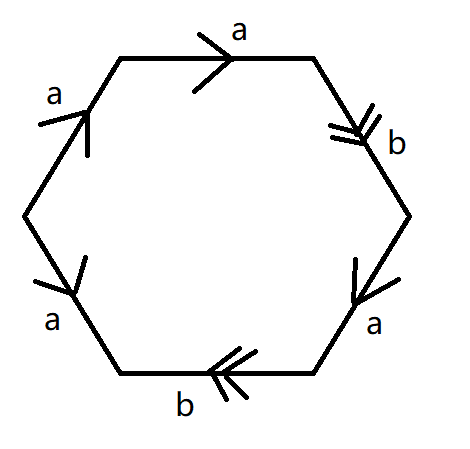
\includegraphics[scale=0.5]{Pictures/HW2-6-1.png}\]
\begin{enumerate}[(a)]
\item Calculate the homology and cohomology groups of \(X\) with \(\mathbb{Z}/2\)-coefficients. 
\item Give a \(\Delta\)-complex structure to \(X\), for example by placing one point in the center of the hexagon, drawing lines to the outer vertices, and orienting the \(2\)-simplices 
appropriately.
\item Using your \(\Delta\)-complex structure, give a \(1\)-cocycle \(\alpha\) with \(\mathbb{Z}/2\)-coefficients having the property that \(\alpha(a)=1\) and \(\alpha(b)=0\). 
\item Compute\(\alpha\cup \alpha\) on all the 2-simplices in your picture. Is \(\alpha\cup \alpha\) zero or nonzero in \(H^2(X;\mathbb{Z}/2)\)? Explain. 
\end{enumerate}
\end{problem}
\begin{solution}
\begin{enumerate}[(a)]
\item Consider the following celluar structure of \(X\)
\[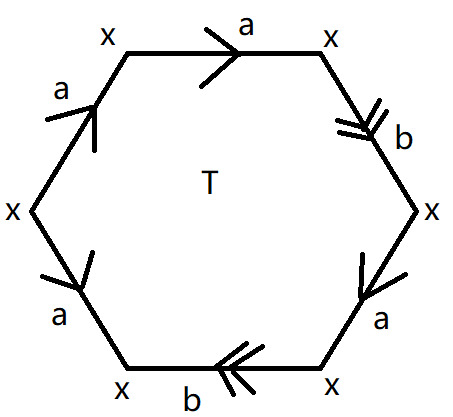
\includegraphics[scale=0.5]{Pictures/HW2-6-2.png}\]
\(X\) has one \(0\)-cell \(x\), two \(1\)-cell \(a,b\) and one \(2\)-cell \(T\). We have a cellular chain complex with coefficients \(\mathbb{Z}/2\)
\[0\rightarrow \mathbb{Z}/2\xrightarrow{0}(\mathbb{Z}/2)^2\xrightarrow{0}\mathbb{Z}/2\rightarrow 0\]
Note that all boundary maps are \(0\), so apply \(\hom(-,\mathbb{Z}/2)\) will obtain all \(0\) coboundary maps. This implies 
\begin{multicols}{2}
\noindent
\[H_i(X;\mathbb{Z}/2)=\begin{cases}
    \mathbb{Z}/2,&\iif i=0,2;\\ 
    (\mathbb{Z}/2)^2,&\iif i=1;\\ 
    0,&\otherwise.
\end{cases}\]
\noindent 
\[H^i(X;\mathbb{Z}/2)=\begin{cases}
    \mathbb{Z}/2,&\iif i=0,2;\\ 
    (\mathbb{Z}/2)^2,&\iif i=1;\\ 
    0,&\otherwise.
\end{cases}\]
\end{multicols}
\item The following is a \(\Delta\)-complex structure on \(X\)
\[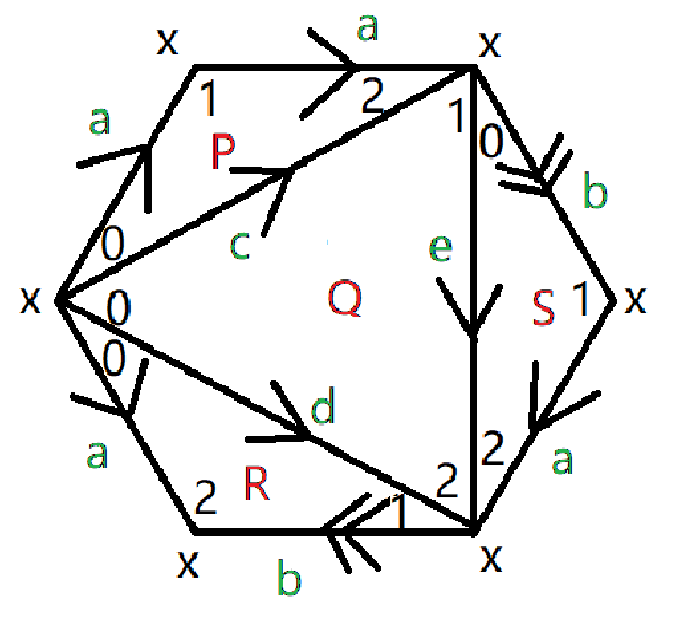
\includegraphics[scale=0.4]{Pictures/HW2-6-3.png}\]
\item Consider the \(1\)-cochain \(\alpha=\hat{a}+\hat{d}+\hat{e}\) satisfying \(\alpha(a)=1\) and \(\alpha(b)=0\). Let us check this is a cocycle. 
\begin{align*}
 \delta(\hat{a}+\hat{d}+\hat{e})(P)&=(\hat{a}+\hat{d}+\hat{e})(a+a-c)=1+1=0,\\ 
 \delta(\hat{a}+\hat{d}+\hat{e})(Q)&=(\hat{a}+\hat{d}+\hat{e})(c+e-d)=1+1=0,\\ 
 \delta(\hat{a}+\hat{d}+\hat{e})(S)&=(\hat{a}+\hat{d}+\hat{e})(b+a-e)=1+1=0,\\ 
 \delta(\hat{a}+\hat{d}+\hat{e})(R)&=(\hat{a}+\hat{d}+\hat{e})(a-b-d)=1+1=0.
\end{align*}
This proves \(\alpha=\hat{a}+\hat{d}+\hat{e}\) is a \(1\)-cocycle satisfying \(\alpha(a)=1\) and \(\alpha(b)=0\).
\item We calculate \(\alpha\cup \alpha\) on each 2-simplices. 
\begin{align*}
    (\alpha\cup\alpha)(P)&=\alpha(a)\cdot \alpha(a)=1\cdot 1=1,\\ 
    (\alpha\cup \alpha)(Q)&=\alpha(c)\cdot \alpha(e)=0\cdot 1=0,\\ 
    (\alpha\cup\alpha)(S)&=\alpha(b)\cdot \alpha(a)=0\cdot 1=0,\\ 
    (\alpha\cup\alpha)(R)&=\alpha(d)\cdot \alpha(b)=1\cdot 0=0. 
\end{align*}
This proves that \(\alpha\cup\alpha=\hat{P}\) on the chain level. Suppose \(\sigma\in C^1(X;\mathbb{Z}/2)\) satisfying \(\delta\sigma=\hat{P}\). Then we have 
\begin{align*}
    (\delta\sigma)(P)&=\sigma(c)=1,\\ 
    (\delta\sigma)(Q)&=\sigma(c)+\sigma(e)+\sigma(d)=0,\\ 
    (\delta\sigma)(S)&=\sigma(b)+\sigma(a)+\sigma(e)=0,\\ 
    (\delta\sigma)(R)&=\sigma(a)+\sigma(b)+\sigma(d)=0.
\end{align*}
We add the last two equations together and obtain 
\[\sigma(e)+\sigma(d)=0\]
But from the second and first equation, we know that \(\sigma(e)+\sigma(d)+1=0\). This leads to a contradiction, so \(\alpha\cup\alpha=\hat{P}\) is not a coboundary, thus \([\alpha\cup\alpha]\neq 0\) in \(H^*(X;\mathbb{Z}/2)\).
\end{enumerate}
\end{solution}





\end{document}